\documentclass[Royal,times,sageh]{sagej}

\usepackage{moreverb,url,natbib, multirow, tabularx}
\usepackage[colorlinks,bookmarksopen,bookmarksnumbered,citecolor=red,urlcolor=red]{hyperref}



% tightlist command for lists without linebreak
\providecommand{\tightlist}{%
  \setlength{\itemsep}{0pt}\setlength{\parskip}{0pt}}



\usepackage[linesnumbered,lined,boxed,commentsnumbered]{algorithm2e}
\usepackage{booktabs}
\usepackage{longtable}
\usepackage{array}
\usepackage{multirow}
\usepackage{wrapfig}
\usepackage{float}
\usepackage{colortbl}
\usepackage{pdflscape}
\usepackage{tabu}
\usepackage{threeparttable}
\usepackage{threeparttablex}
\usepackage[normalem]{ulem}
\usepackage{makecell}
\usepackage{xcolor}


\begin{document}


\setcitestyle{aysep={,}}

\title{A geo-referenced micro-data set of real estate listings for
Spain's three largest cities}

\runninghead{author \emph{et al}.}

\author{\affilnum{}}

\affiliation{}



\begin{abstract}
This article presents an open data product with large geo-referenced
micro-data sets of 2018 real estate listings in Spain. These data were
originally published on the idealista.com real estate website. The
observations were obtained for the three largest cities in Spain: Madrid
(n = 94,815 observations), Barcelona (n = 61,486 observations), and
Valencia (n = 33,622 observations). The data sets include the
coordinates of properties (latitude and longitude), asking prices of
each listed dwelling, and several variables of indoor characteristics.
The listings were enriched with official information from the Spanish
cadastre (e.g., building material quality) plus other relevant
geographical features, such as distance to urban points of interest.
Along with the real estate listings, the data product also includes
neighborhood boundaries for each city. The data product is offered as a
fully documented R package and is available for scientific and
educational purposes, particularly for geo-spatial studies
\end{abstract}

\keywords{Housing prices; hedonic price analysis; idealista.com;
geo-referenced data; point-level data; open data; Spain}

\maketitle

\hypertarget{introduction}{%
\section{Introduction}\label{introduction}}

Interest in the characteristics of the housing market and housing prices
has been a growing area of research in recent decades, generating a vast
amount of theoretical and empirical literature. Including the spatial
component to analyze the real estate market and incorporating geographic
variables has significantly improved the understanding of this market:
to this end, it is essential to have information/data at the point
level. Therefore, it is becoming common for spatial analysis of urban
environments to be use micro-data, geo-referenced as points
\citep{lopez2015}. In some cases, researchers have had to resort to
webscraping processes to obtain data for research
\citep[e.g.,][]{gupta2022take, arbia2020spatial, Li2019, lopez2015}.
Alas, webscraping is a chancy process prone to download errors, missing
data, duplicated records, etc. Furthermore, researchers do not always
share their webscrapped datasets, which limits reproducibility of their
research. As we witness a growing interest in openness and
reproducibility in geographical data science
\citep{arribasl2021editorial, paez2021open, brunsdon2021opening}, it
becomes increasingly urgent to have open data products to support
research \citep{arribas2021}.

Some researchers have already responded to this need for publicly
available, geo-referenced datasets to support open, reproducible
research. A few such datasets are now available to support the analysis
of real estate markets, but they are sometimes geo-referenced at the
level of large geographical zones, such as \citet{fuerst2020real}, an
open dataset that includes \(n=4,201\) property prices geocoded to the
level of nine regions in England and Wales. Other datasets are geo-coded
as points, including \citet{bonifaci2015real}, which includes
\(n=1,042\) observations for Padua, in Italy;
\citet{delgiudice2018housing}, who share a dataset with \(n=576\)
observations relating to rental prices in Naples, Italy; and
\citet{solano2019dataset} present a dataset with \(n=1,623\) daily
rental prices in Seville, Spain.

To contribute to the growing inventory of international micro-data sets
of real estate markets, this paper introduces an open micro-data set of
geo-referenced dwelling listings. The data have been provided by the
Idealista
company\footnote{Idealista is the major real estate listing website in Spain, and present in other southern european countries as Italy and Portugal}
and contain information about 189,923 dwellings located in Spain's three
largest cities. To date, this data product is one of the largest open
geo-referenced micro-data set of the housing market in the world. The
most similar in terms of geographical disaggregation and sample size is
the dataset of \citet{song2021hedonic} which includes transactions for
four cities in South Korea, namely Busan (\(n=61,152\)), Daegu
(\(n=32,363\)), Daejeon (\(n=21,114\)), and Gwangju (\(n=25,984\)). It
is certainly the largest in Spain.

The data set has been supplied directly by Idealista, and therefore is
clean and free of download errors. However, to comply with data
legislation, to share the data we have slightly modified the prices by
applying a small amount of random noise which will not bias the main
results derived from its usage.

This micro-data set can be used to benchmark new analytical methods in a
reproducible fashion. Applied and theoretical researchers on real estate
mass appraisal and valuation methods might use this dataset to
canonically compare the performance of their proposed comparable and
hedonic models, among others. The data can also be used to study the
segmentation of housing submarkets and related topics such as the impact
of suburban areas on house prices. The listings have been enriched with
official information from the Spanish cadastre along with other relevant
geographical features, such as distance to urban points of interest. In
any case, the data might be easily extended by spatially joining other
datasets that contain information at administrative, census tract, or
postal code levels.

The data set is distributed as an \texttt{R} package, named
\{idealista18\}, which can be accessed from a public Github
repository\footnote{\url{https://github.com/paezha/idealista18}}. The
open data product is made available under the
\href{http://opendatacommons.org/licenses/odbl/1.0/}{Open Database License}.
For transparency, we also share the randomization process applied to the
original data in the aforementioned Github repository.

\hypertarget{data-description}{%
\section{Data description}\label{data-description}}

The open data product \{idealista18\} is an \texttt{R} package composed
of ten objects, three objects for each of the three main Spanish cities:
Barcelona, Madrid, and Valencia. For each city, dwelling listings,
neighborhood polygons, and a set of points of interest have been
included in the package. There is in addition a data object with the
number of dwellings by district (a collection of neighborhoods),
according to the Spanish cadastre.

The data provider (idealista.com) is a leading real estate portal in
Spain, on par with its nearest competitor Fotocasa. Smaller listing
portals include Habitaclia and Milanuncios, the latter focusing almost
exclusively on individual (i.e., non-professional) advertisers. In
September 2021, according to data from Similarweb (a site specialized in
sites' traffic volume comparison), there were a total of 103 million
page views on real estate portals in Spain. Of this, 94\% of traffic was
concentrated on four portals, of which idealista was the most important,
followed by Fotocasa, Habitaclia, and Pisos.com. Traffic is also highly
concentrated, and idealista.com was the the leader by far with 58.6
monthly million visits (57\% of the total traffic) compared to its
closest competitor with 19.9 million visits (19.3 \% of total traffic).

As a result of its share of advertisments, idealista.com covers fairly
well all segments of the Spanish market, including both individual and
professional advertisers. This dataset includes information about
listing prices, and therefore represents the market situation from the
perspective of asking prices. This is a necessary compromise in the
present case, since actual sale prices are not publicly available, and
the information can only be accessed by paying high fees to Colegio de
Registradores. However listing prices reflect quite well the
(transaction) reality of real estate markets, and correlations between
idealista listings and transaction prices can be established see
\href{https://papers.ssrn.com/sol3/papers.cfm?abstract_id=3400031}{Banco
de España}. Official transactions and asking prices can be taken as
complementary and are of great interest when studying asking-transaction
price gaps or the relation between listing site demand variables (i.e.,
ad contacts or ad views) and price gaps.

To provide some context about the coverage of the \{idealista18\}
dataset Table \ref{tab:transactions} shows the number of listings with
respect to the total residential stock in each city in 2018. As seen in
the table, the number of listings ranges between 6.1\% of the total
number of properties (in Madrid) and 8.1\% (in Valencia). Information
from Instituto Nacional de Estadistica\footnote{\url{https://www.ine.es/jaxiT3/Tabla.htm?t=6150&L=1}}
shows that the number of listings in the \{idealista18\} package
correspond to 81.3\% of recorded real estate transactions in Barcelona,
80.8\% in Madrid, and 91.1\% in Valencia.

\begin{table}[!ht]
    \centering
      \caption{Total properties and transactionst three Spanish cities. Year 2018} 
  \label{tab:transactions} 
    \begin{tabular}{lccccc}
        City & Total properties (P) & Total transactions (T) & Listings (L) & L/P & T/L \\
        \hline
        Barcelona &  789,740  &  56,012  &  61,329  & 7.8\% & 81.3\%  \\ 
        Madrid &  1,545,397  &  76,603  &  94,802  & 6.1\%  & 80.8\% \\ 
        Valencia &  416,004  &  30,615  &  33,593  & 8.1\% & 91.1\% \\ 
        \hline
        Total &  2,751,141  &  163,230  &  189,724  & 6.9\% & 86.0\% \\ 
        \hline
        \multicolumn{6}{l}{{\footnotesize \textbf{Sources}}}\\
        \multicolumn{6}{l}{{\footnotesize Total properties (P): Ministerio Español de Hacienda y Función Pública}}\\
        \multicolumn{6}{l}{{\footnotesize Total transactions (T): Instituto Nacional de Estadística}}\\
    \end{tabular}
\end{table}

The following subsections describe each object. A full description of
the data is available in the help section of the package. We have tried
to the best of our ability to comply with FAIR principles regarding
research data \citep{Wilkinson2016fair}: upon publication, the dataset
has a persistent digital object identifier; publication as a data
article makes the data findable; the data and metadata are packaged
together and protocols for help files in the R ecosystem mean that
documentation is easily searchable; distribution as an R package means
that only open software is needed to access the data; and a public
repository documents all data processes followed to generate the
distributed open data product.

\hypertarget{dwelling-listings}{%
\subsection{Dwelling listings}\label{dwelling-listings}}

The dwelling listing of each city includes a set of characteristics for
each dwelling published on the idealista real estate website as an ad.
The dwelling listing has been included in the \{idealista18\} package as
a simple features (sf) object \citep{Pebesma} with point geometry in
latitude and longitude. The name of each sf object with the list of
dwellings is the name of the city followed by '\_Sale' (e.g.,
Madrid\_Sale). Each data object includes a total of 42 variables and the
complete set of listings corresponding to the four quarters of 2018.
Table \ref{tab:number-ads} shows the number of dwelling listing ads
included in the data set for each city and quarter. The record counts
for each city are: 94,815 listings for Madrid, 61,486 for Barcelona, and
33,622 for Valencia. Note that the same dwelling may be found in more
than one period when a property listed for sale in one quarter was sold
in a subsequent quarter. The variable ASSETID, included in the sf
objects, is the unique identifier of the dwelling.

\begin{table}[ht]
\centering
\begin{tabular}{>{\raggedright\arraybackslash}p{4em}>{\raggedleft\arraybackslash}p{3em}cccc}
  \hline
City$\backslash$Quarter & First & Second  & Third & Fourth & Total ads \\ 
  \hline
Barcelona & 17826 & 7951 & 12375 & 23334 & 61486 \\ 
  Madrid & 21920 & 12652 & 15973 & 44270 & 94815 \\ 
  Valencia & 9305 & 4655 & 5644 & 14018 & 33622 \\ 
   \hline
\end{tabular}
\caption{Number of dwelling  listing ads for each city and quarter. \label{tab:number-ads}} 
\end{table}

Each record of the dwelling listing contains a set of indoor
characteristics supplied by the advertisers on the Idealista website
(e.g., price, surface area, number of bedrooms, basic features, etc.),
including the location of the dwelling. The exact location has been
masked, as described in Section
\protect\hyperlink{anonymizing}{Anonymizing the data set}). Table
\ref{tab:variables} lists the main indoor variables with a short
description and the mean value of each variable. The dwelling listings
were enriched with a number of additional attributes from the Spanish
cadastre \citep{Catastro}. The cadastral information is described in
Table \ref{tab:variables}, with the prefix CAD in the variable name. The
cadastral features were assigned by applying the features of the nearest
parcel to the coordinates. The year the dwelling was built
(CONSTRUCTIONYEAR) given by the advertiser was revised since the year of
construction is entered on the website by users, and it is therefore
subject to errors and incomplete data (40\% missing data). To resolve
this issue, an alternative variable (CADCONSTRUCTIONYEAR) was included,
assigning the cadastral construction year from the nearest cadastral
parcel whenever the value was outstanding (date was after publication
date or year of construction was before 1500) or when the value supplied
by the advertiser was missing.

Additionally, the distance of each dwelling to several points of
interest was included in the sf object: distance to the city center,
distance to the closest metro station, and distance to a major street
(La Diagonal for Barcelona, La Castellana for Madrid, and Blasco Ibañez
for Valencia). The last rows of Table \ref{tab:variables} show the mean
values of these variables.

\begin{table}[ht]
\centering
\fontsize{8}{10}\selectfont
\begin{tabular}{>{\raggedright\arraybackslash}p{13em}>{\raggedright\arraybackslash}p{14em}ccc}
  \hline
Variable & Sort Description & Barcelona & Madrid & Valencia \\ 
  \hline
PRICE & Asking price & 395770.58 & 396110.11 & 199678.31 \\ 
  UNITPRICE & Asking price per m\verb|^|2 (euros) & 4044.86 & 3661.05 & 1714.54 \\ 
  CONSTRUCTEDAREA & Surface (m\verb|^|2) & 95.46 & 101.40 & 108.95 \\ 
  ROOMNUMBER & Number of bedrooms & 2.86 & 2.58 & 3.07 \\ 
  BATHNUMBER & Number of bathrooms & 1.52 & 1.59 & 1.59 \\ 
  CONSTRUCTIONYEAR & Construction year (advertiser) & 1952.58 & 1964.69 & 1969.43 \\ 
  CADCONSTRUCTIONYEAR & Construction year (cadastre) & 1952.19 & 1965.70 & 1970.55 \\ 
  CADMAXBUILDINGFLOOR & Max build floor & 6.85 & 6.38 & 7.04 \\ 
  CADDWELLINGCOUNT & Dwelling count in the building & 28.56 & 39.19 & 36.83 \\ 
  CADASTRALQUALITYID & Cadastral quality. 0 Best-10 Worst & 4.31 & 4.85 & 5.34 \\ 
  DISTANCE\_TO\_CITY\_CENTER & Distance to city center & 2.80 & 4.49 & 2.09 \\ 
  DISTANCE\_TO\_METRO & Distance to subway station & 0.27 & 0.48 & 0.64 \\ 
  DISTANCE\_TO\_(MAINSTREET) & Distance to major street & 1.77 & 2.68 & 2.07 \\ 
   \hline
\end{tabular}
\caption{List, sort description, and mean of the main quantitative variables included in the dwelling listing for the three Spanish cities. See the help section in the \textbf{idealista18} R package for details and formal definitions. Some variables have been excluded from this table to save space. Check the full list in the \textbf{idealista18} package.\label{tab:variables}} 
\end{table}

In addition to the variables listed in Table \ref{tab:variables}, the sf
object includes a set of dummy variables with information about the
basic characteristics of the dwelling. Table \ref{tab:Dummy-variables}
shows the more relevant variables included in the sf object.

\begin{table}[ht]
\centering
\fontsize{8}{10}\selectfont
\begin{tabular}{>{\raggedright\arraybackslash}p{12em}>{\raggedright\arraybackslash}p{14em}ccc}
  \hline
Variable & Sort Description & Barcelona & Madrid & Valencia \\ 
  \hline
HASTERRACE & =1 if has terrace & 0.33 & 0.36 & 0.25 \\ 
  HASLIFT & =1 if has lift & 0.74 & 0.70 & 0.79 \\ 
  HASAIRCONDITIONING & =1 if has air conditioning & 0.47 & 0.45 & 0.47 \\ 
  HASPARKINGSPACE & =1 if has parking & 0.08 & 0.23 & 0.17 \\ 
  HASNORTHORIENTATION & =1 if has north orientation & 0.13 & 0.11 & 0.13 \\ 
  HASSOUTHORIENTATION & =1 if has south orientation & 0.31 & 0.24 & 0.19 \\ 
  HASEASTORIENTATION & =1 if has east orientation & 0.24 & 0.20 & 0.25 \\ 
  HASWESTORIENTATION & =1 if has west orientation & 0.16 & 0.15 & 0.15 \\ 
  HASBOXROOM & =1 if has boxroom & 0.12 & 0.26 & 0.13 \\ 
  HASWARDROBE & =1 if has wardrobe & 0.30 & 0.57 & 0.53 \\ 
  HASSWIMMINGPOOL & =1 if has swimmingpool & 0.03 & 0.15 & 0.07 \\ 
  HASDOORMAN & =1 if has doorman & 0.08 & 0.25 & 0.05 \\ 
  HASGARDEN & =1 if has garden & 0.04 & 0.18 & 0.06 \\ 
  ISDUPLEX & =1 if is duplex & 0.03 & 0.03 & 0.02 \\ 
  ISSTUDIO & =1 if is studio & 0.02 & 0.03 & 0.01 \\ 
  ISINTOPFLOOR & =1 is on the top floor & 0.02 & 0.02 & 0.01 \\ 
  BUILTTYPEID\_1 & =1 if is new contruction & 0.01 & 0.03 & 0.03 \\ 
  BUILTTYPEID\_2 & =1 is second hand to be restored & 0.17 & 0.19 & 0.13 \\ 
  BUILTTYPEID\_3 & =1 is second hand in good condition & 0.82 & 0.78 & 0.83 \\ 
   \hline
\end{tabular}
\caption{List of dummy variables, sort description, and ratios of dwellings with the specific characteristics. See the help section in the \textbf{idealista18} R package for details and formal definitions. Some dummy variables have been excluded from this table to save space\label{tab:Dummy-variables}} 
\end{table}

\hypertarget{neighboorhood-polygons}{%
\subsection{Neighboorhood polygons}\label{neighboorhood-polygons}}

The second data object included in \{idealista18\} is the neighborhoods
in the three cities as polygons. There is an sf object for each city
with the name of the city and the suffix '\_Polygons'. Figure
\ref{fig:all-polygons} shows the quantile maps of the number of
dwellings in the listing for the different neighborhoods in the three
cities. The neighborhoods are based on the official boundaries but
slightly changed by
Idealista\footnote{There are two criteria used to make this division. If an area is small enough and similar enough to another, the two areas are merged, and, if the official area is not homogeneous, it is divided into a series of new polygons.}.
In practical terms, we can assume they are the same since the website
combines areas when there are few ads for that area. In the case of
Madrid, they combined four areas into two.

\begin{figure}
\centering
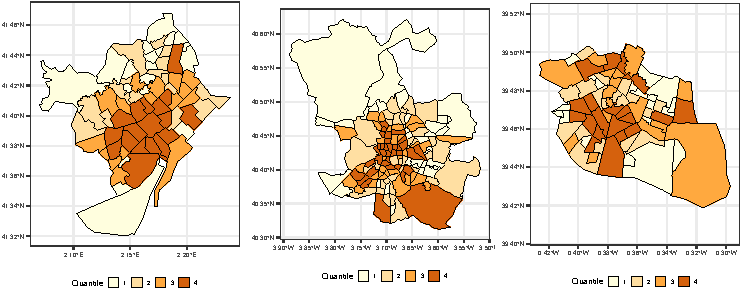
\includegraphics{main_EPB_files/figure-latex/unnamed-chunk-1-1.pdf}
\caption{\label{fig:all-polygons}Number of listings in each
neighborhood. Boundary for Barcelona (Top), Madrid (Center), and
Valencia (Bottom).}
\end{figure}

There are a total of 69 neighborhoods in Barcelona, 135 in Madrid, and
73 in Valencia. The sf object includes a unique identifier (LOCATIONID)
and the neighborhood name (LOCATIONNAME).

The total number of dwellings is available from the Spanish cadastre
aggregated by district (districts are groups of neighborhoods). Figure
\ref{fig:districts} shows the percentage of listed dwellings relative to
the total number of dwelling by district in each of the three cities.
This gives a sense of how active residential real estate markets were in
different parts of each city in 2018.

\begin{figure}
\centering
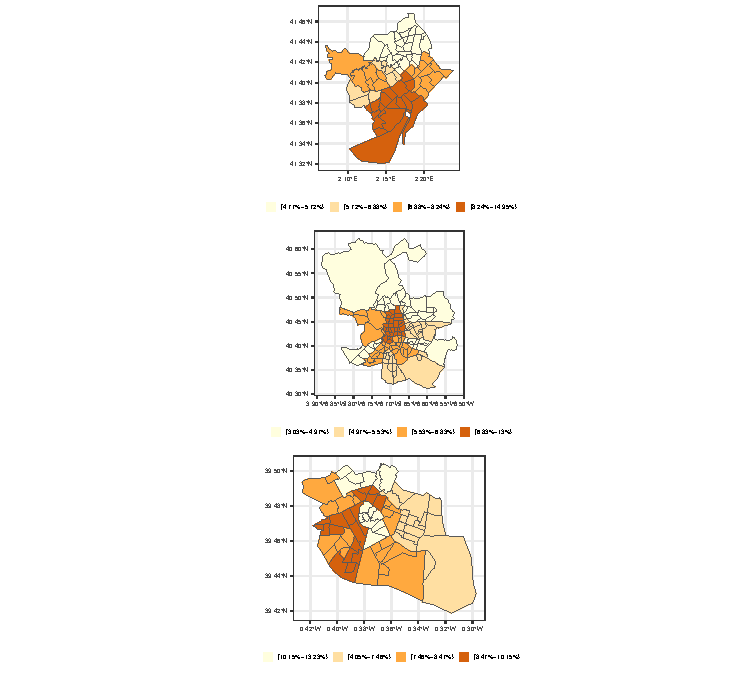
\includegraphics{main_EPB_files/figure-latex/unnamed-chunk-2-1.pdf}
\caption{\label{fig:districts}Percentage of listings relative to total
number of dwellings by district. Boundary for Barcelona (Top), Madrid
(Center), and Valencia (Bottom).}
\end{figure}

\hypertarget{points-of-interest}{%
\subsection{Points of Interest}\label{points-of-interest}}

The last data object included in the package is a set of Points of
Interest in each city as an object of the class list. The name of the
list includes the name of the city with the suffix '\_POIS'. These lists
include three elements: (i) the coordinates of the city center, the
central business district; (ii) a set of coordinates that define the
main street of each city; and (iii) the coordinates of the metro
stations.

\hypertarget{anonymizing}{%
\section{Anonymizing the data set}\label{anonymizing}}

To comply with Spanish regulations, two variables were slightly modified
to provide anonymity. A masking process was applied to asking prices and
location (coordinates).

In terms of the asking prices, the original values were obfuscated with
the addition or subtraction of a random percentage of their original
values, ranging from \(-2.5%
\) to \(+2.5%
\). Since asking prices are usually multiples of 1,000, after the first
price modification, the prices were aligned to multiples of 1,000.

\begin{algorithm}[!ht]
 \KwData{all idealista listings}
 \KwResult{all idealista listings with masked coordinates}
 initialization\;
 \For{each listing L}{
  take geographical location of L as $(X,Y)$
  \Repeat{this stop condition}{
    take a random angle $\alpha$ from 0 to 360 degrees
    take a distance $R$ as a random value from 30 to 60 meters
    determine a new point $(X',Y')$ calculated as a point located $R$ with the angle $\alpha$
  }
  set $(X',Y')$ as the new location for the listing L
 }
 \caption{Coordinate displacement process for anonymisation purposes}
 \label{algo:coordinates-displacement}
\end{algorithm}

With respect to the location of the dwelling, a spatial masking process
was implemented to maintain the spatial properties of the original data
set. The coordinates of each listing were displaced using a stochastic
procedure. The listings were recorded using coordinates contained in
maximum and minimum displacement circles, as shown in Figure
\ref{fig:Anonymizing} (left). To preserve inclusion in a neighborhood,
the spatial masking procedure was constrained to ensure that the masked
coordinates remained in the original neighborhood of the listing.

Algorithm \ref{algo:coordinates-displacement} iteratively displaces the
coordinates of each listing with a minimum distance and a maximum
distance with the restriction that the new coordinates do not fall into
a different neighborhood. This ensures that neighborhood attributes are
preserved.

Figure \ref{fig:Anonymizing} (right) shows the histogram of the
displacements in meters for all the listings in the city of Valencia.
The average distance between the original and masked coordinates is 45
meters.

\begin{figure}

{\centering 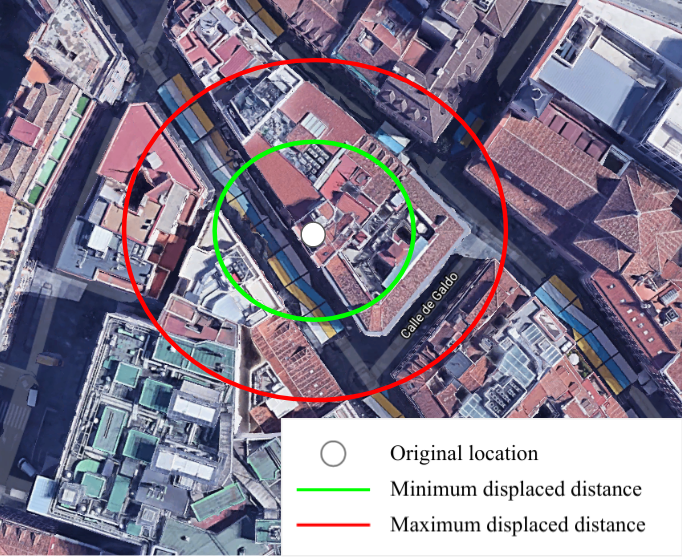
\includegraphics[width=0.29\linewidth,height=0.2\textheight]{EPB_files/points-moved-image} 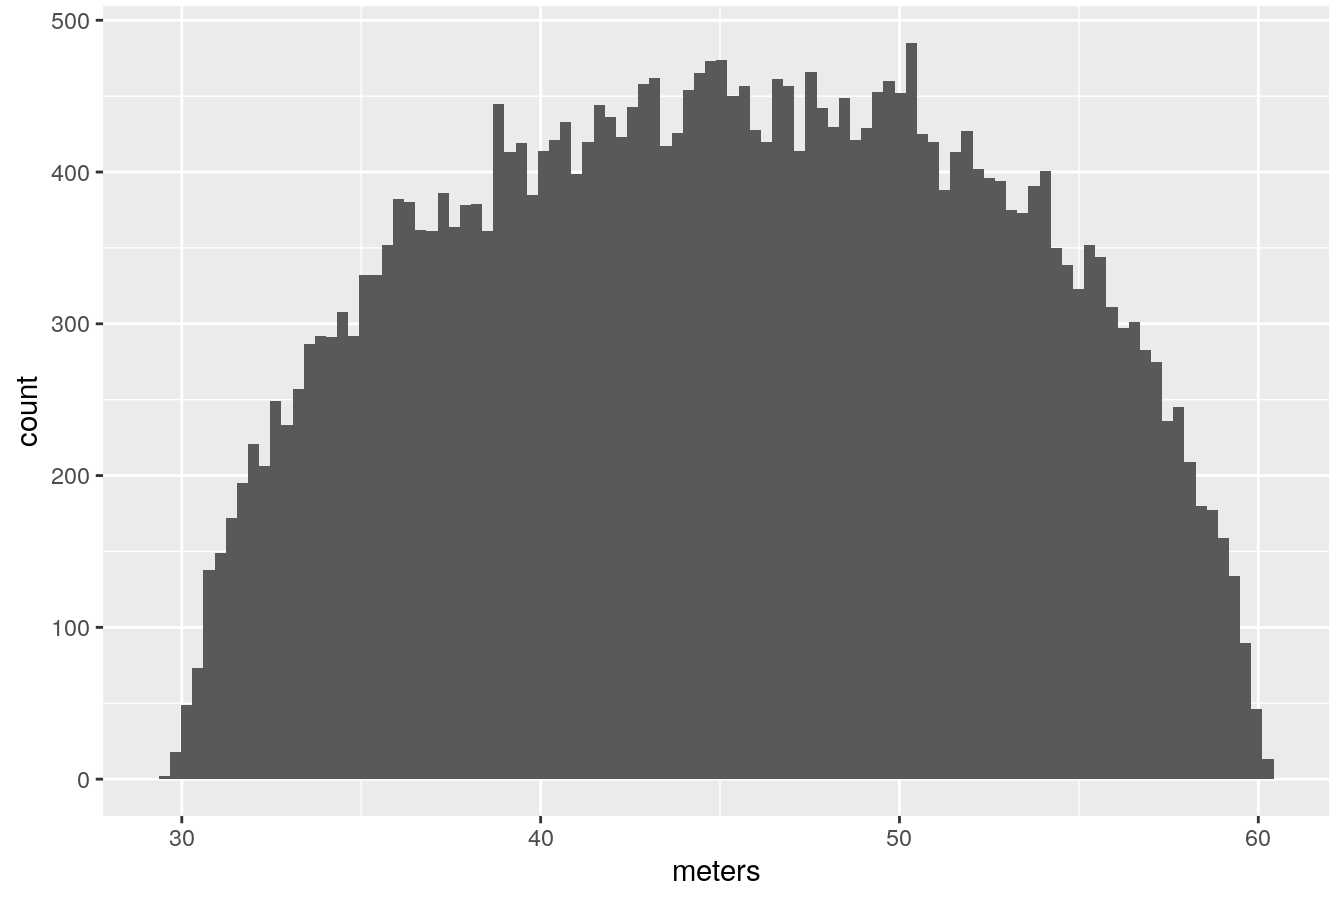
\includegraphics[width=0.37\linewidth,height=0.2\textheight]{EPB_files/coordinates-valencia} 

}

\caption{\label{fig:Anonymizing}(Left) Masking coordinates. Spatial range. (Right) Coordinate displacement in meters (Valencia)}\label{fig:unnamed-chunk-3}
\end{figure}

\hypertarget{conclusion}{%
\section{Conclusion}\label{conclusion}}

This paper describes a data product of a geo-referenced micro-data set
of Spain's three largest cities. This is an excellent data product to
help understand the complex mechanisms related to the housing market and
housing prices. Researchers can apply hedonic models with spatial
effects, identifying housing submarkets or machine learning techniques
\citep[e.g.,][]{rey2023using}. The data product can also be used for
educational proposes and teaching activities.

\hypertarget{declaration-of-competing-interest}{%
\section{Declaration of Competing
Interest}\label{declaration-of-competing-interest}}

Author One and author Two are employed by Idealista. They have been
granted permission to share the data presented in this article. None of
the authors have financial interests or personal relationships which
have, or could be perceived to have, influenced the work reported in
this article.

\hypertarget{acknowledgments}{%
\section{Acknowledgments}\label{acknowledgments}}

The authors wish to thank Alessandro Galesi for their support in the
paper revision and Juan Ramón Selva for collecting and cleaning the
spatial data. This work has been partially funded by the Spanish
Ministry of Economy and Competitiveness Grants PID2019-107800GB-100

\bibliographystyle{sageh}
\bibliography{bibEPB.bib}


\end{document}
